\paragraph{Span}
It plays a role like that of the tuning parameter $\lambda$ in 
smoothing splines: \tB{it controls the flexibility of the non-linear fit}.\\
\sT{The smaller the value of $s$, the more \emph{local} will be our fit.}

\paragraph{Algorithm: \emph{Local Regression} at $X=x_{0}$}
\begin{figure}[H]
	\begin{center}
		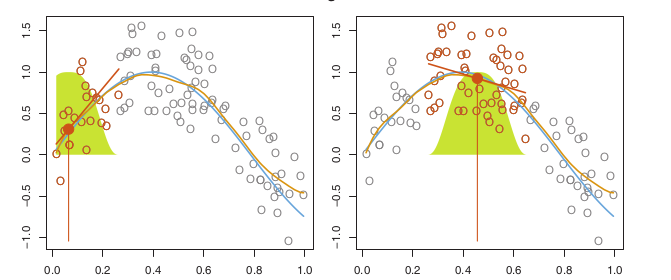
\includegraphics[width=\textwidth]{./chap/1chap/6sec/images/2localRegression.png}
	\end{center}
	\caption{Blue curve represents $f(x)$ from which the data were
	generated.\\
	Orange curve corresponds to the local regression estimate $f(x)$.\\
	Orange colored points are local to the target point $x_{0}$.\\
	Yellow-bell-shape superimposed on the plot indicates weights 
	assigned to each point, decreasing to zero with distance from
	the target point.}
	\label{fig:6.1localRegression}
\end{figure}
\begin{enumerate}
	\item Gather the fraction $s=\frac{k}{n}$ of training points
		whose $x_{i}$ are closet to $x_{0}$
	\item Assign a weight $k_{i0}=K(x_{i},x_{0})$ so that \tB{the
		point furthest from $x_{0}$ has weight zero, and the 
		closet has the highest weight}.\\
		\sB{All but these $k$ nearest neighbors get weight 0}
	\item \tB{Fit a weighted least squares regression of the $y_{i}
		$ on the $x_{i}$}, using the aforementioned weights, by
		\tB{finding $\beta_{0}$ and $\beta_{1}$ that minimize:
		$$\su{{i=1}}{n}K_{i0}(y_{i}-\beta_{0}-\beta_{1}x_{i})^{2}$$}
	\item \tB{The fitted value at $x_{0}$ is given by $\hat{f}(x_{
		0})= \hat{\beta}_{0}+\hat{\beta}_{1}x_{0}$}
\end{enumerate}
For $p$-dimensional neighborhoods, local regression can perform poorly
if $p$ is much larger than 3 or 4, because there will generally be very
few training observations close to $x_{0}$
